\documentclass{article}

% Use the COLM 2026 conference style (submission mode = anonymous)
\usepackage[submission]{colm2026_conference}

% Configure natbib for numbered citations
\setcitestyle{numbers,square}

% Standard packages
\usepackage{times}
\usepackage{graphicx}
\usepackage{amsmath,amsfonts,amssymb}
\usepackage{booktabs}
\usepackage{multirow}
\usepackage{algorithm}
\usepackage{algorithmic}
\usepackage{tikz}
\usepackage{pgfplots}
\pgfplotsset{compat=1.18}
\usetikzlibrary{shapes,arrows,positioning,calc,patterns}

% Math commands
\input{math_commands}

% Hyperref for cross-references (but not visible URLs in submission mode)
\usepackage[hidelinks]{hyperref}

% Title and authors (anonymized for submission)
\title{Agent Memory Below the Prompt: \\
Persistent Q4 KV Cache for Multi-Agent LLM Inference on Edge Devices}

% Anonymous submission
\author{Anonymous Authors}

\begin{document}

\maketitle

\begin{abstract}
Multi-agent LLM workflows on Apple Silicon spend most of their time re-computing attention state. A 5-agent system with 4K tokens each waits 77 seconds after every server restart while each agent re-prefills from scratch. We persist each agent's KV cache to disk in 4-bit quantized format and reload it in under 700\,ms. Three components make this work: (1)~a block pool giving each agent an isolated, persistent Q4 KV cache stored in safetensors, (2)~BatchQuantizedKVCache for concurrent inference over multiple agents' quantized caches, and (3)~cross-phase context injection that lets agents accumulate attention state across conversation phases without re-computation. On Gemma~3 12B and DeepSeek-Coder-V2-Lite 16B at typical deployment lengths (4K context), warm disk reload reduces TTFT from 15.5s to 513\,ms (30$\times$) and from 3.9s to 252\,ms (16$\times$). At 32K context, the speedup reaches 130$\times$ and 74$\times$. Batched serving of two concurrent agents reaches 22.4 and 64.8 system tokens/second with warm cache. Q4 quantization fits 3.6$\times$ more agent contexts into fixed device memory than FP16, with $<$0.1 perplexity degradation. The system handles both dense GQA (Gemma) and MoE MLA (DeepSeek) architectures through a model-agnostic abstraction, and operates as an infrastructure layer beneath agentic frameworks (AutoGen, CrewAI) via its OpenAI-compatible API. Open-source at \texttt{[anonymized]}.
\end{abstract}

\section{Introduction}
\label{sec:intro}

Five agents, each holding 4,096 tokens of conversation history. The server restarts. On an Apple M4~Pro, each agent needs 15.5 seconds to re-prefill its context through the model. Total: 77 seconds of dead time before any agent can respond.

This is the cold-start problem for multi-agent LLM inference on edge devices. Datacenter GPUs process tokens at 10,000+/second, making a 4K re-prefill a 400\,ms annoyance. Apple Silicon processes them at roughly 260/second (Gemma~3 12B, M4~Pro). The gap is 40$\times$.

The problem is worse than slow prefill. Each agent needs its own attention context. Concatenating multiple agents' histories into one long prompt introduces position bias: information in the middle of long sequences gets less attention than information at the start or end~\cite{liu2024lost}. Separate KV caches per agent avoid this, but $N$ agents with $C$ tokens each require $N \times C$ tokens of cache memory on a device where RAM is soldered and fixed.

We eliminate re-prefill by persisting each agent's KV cache. The cache produced during prefill is the agent's memory at the attention layer. Instead of discarding it after each request (as vLLM~\cite{kwon2023pagedattention} and SGLang~\cite{zheng2024sglang} do) or holding it only in volatile RAM, we write it to disk in 4-bit quantized format and reload it when the agent resumes. Context restoration drops from 15.5 seconds to 513\,ms (warm, disk) or 709\,ms (hot, memory) at 4K context on Gemma~3 12B.

\paragraph{Contributions.} (1)~A persistent block pool giving each agent isolated, quantized KV cache surviving server restarts and device reboots, stored in safetensors format. (2)~BatchQuantizedKVCache for concurrent Q4 inference over multiple agents' caches, with an interleaved prefill+decode scheduler. (3)~Cross-phase context injection treating KV cache as working memory, letting agents accumulate attention state across conversation phases without re-computation. (4)~An infrastructure layer for agentic frameworks: the system exposes an OpenAI-compatible API, so AutoGen~\cite{wu2023autogen}, CrewAI, or LangGraph can use persistent cache without modification. (5)~Evaluation across two architecturally distinct models showing Q4 persistence fits 3.6$\times$ more agents than FP16 with negligible quality loss.

\section{Background}
\label{sec:background}

\subsection{The Multi-Agent Memory Problem}
\label{sec:memory_problem}

LLM inference has two phases: prefill (process all input tokens in parallel, producing KV pairs for each attention layer) and decode (generate output tokens one at a time, attending to cached KV state). Prefill is compute-bound. Decode is memory-bandwidth-bound.

Multi-agent systems compound the prefill cost. Each agent requires its own context because attention is quadratic in sequence length: concatenating 5 agents' 4K contexts into one 20K prompt would increase attention cost 25$\times$ compared to separate 4K passes, and would expose answers to position bias~\cite{liu2024lost,jiang2024minference}. Agents in the middle of the concatenated context receive less attention weight. Separate contexts are necessary for unbiased multi-agent inference.

Separate contexts mean separate KV caches. A 5-agent system needs 5 independent caches. Real agentic workflows scale to 5--20+ agents: AutoGen teams, CrewAI crews, and debate architectures each assign specialized roles that require independent conversational state~\cite{guo2024multiagent}. SagaLLM identifies ``context loss'' across agent boundaries as a fundamental limitation of current multi-agent systems~\cite{chang2025sagallm}.

On a datacenter GPU, keeping 20 caches in memory is routine. On an edge device with 24\,GB of fixed RAM, keeping 5 caches requires lifecycle management: which caches to keep hot, which to persist to disk, and when to reload. Without persistence, every agent cold-starts from scratch on every request.

\subsection{Edge Device Constraints}
\label{sec:edge_constraints}

Server GPUs add memory by installing DIMMs. Edge devices ship with soldered DRAM. A 24\,GB Mac Mini will always have 24\,GB. Table~\ref{tab:hardware} shows current edge-class hardware.

\begin{table}[t]
\centering
\small
\caption{Edge device memory and bandwidth. Unified memory devices share RAM between CPU and GPU. Discrete GPUs (RTX) have separate VRAM; KV cache offload to host RAM drops to PCIe bandwidth.}
\label{tab:hardware}
\begin{tabular}{@{}lrrrl@{}}
\toprule
Device & Mem & BW & SSD & Type \\
       & (GB) & (GB/s) & (GB/s) & \\
\midrule
M4 Pro (Mac Mini) & 24 & 273 & 7 & Unified \\
M4 Max (MacBook) & 128 & 546 & 7 & Unified \\
DGX Spark & 128 & 273 & 11 & Unified \\
RTX 5090 (VRAM) & 32 & 1792 & 64$^*$ & Discrete \\
RTX 4090 (VRAM) & 24 & 1008 & 32$^*$ & Discrete \\
iPhone 17 Pro & 12 & 77 & 2 & Unified \\
\bottomrule
\multicolumn{5}{@{}l@{}}{$^*$PCIe host-device bandwidth for KV cache offload.}
\end{tabular}
\end{table}

The RTX 5090 has 1,792\,GB/s bandwidth to its 32\,GB VRAM, but spilling KV cache to host RAM drops to 64\,GB/s (PCIe 5.0), a 28$\times$ cliff. Unified memory devices avoid this penalty but face fixed total capacity. The M4~Pro's internal NVMe reads at 7\,GB/s, which enables sub-second cache reloads for multi-MB KV states.

On our test device (M4~Pro, 24\,GB), the memory budget is 24\,GB $-$ 6.8\,GB weights $-$ 2\,GB OS $\approx$ 15.2\,GB for KV caches. This constrains both the number of concurrent agents and the maximum context length per agent (Section~\ref{sec:fp16_analysis}).

Local inference avoids transmitting conversation history to external servers. Under GDPR (Art.~44--49) and HIPAA (45 CFR 164.312), transferring patient or user data to cloud endpoints requires legal basis, data processing agreements, and transfer impact assessments. On-device inference sidesteps this. The tradeoff: operating within fixed device memory.

\subsection{Interactivity and TTFT}
\label{sec:interactivity}

Response latency determines whether interactive agents feel responsive. Nielsen's thresholds~\cite{nielsen1993} identify 100\,ms as instantaneous, 1\,s as acceptable, and 10\,s as the limit before users disengage. No current local AI system meets the 1\,s threshold at long context~\cite{nielsen2024speed}.

For short multi-turn agent responses (50--200 tokens at ${\sim}$50 tok/s = 1--4\,s decode), prefill dominates perceived latency. At 4K context on Gemma~3, cold prefill is 15.5\,s. Adding 3\,s decode gives 18.5\,s total, of which 84\% is prefill. At shorter outputs (50 tokens, 1\,s decode), prefill is 94\% of latency.

RAG cannot solve this. RAG re-retrieves text chunks and re-runs prefill over them on every request. Prefill accounts for 95.5\% of RAG inference time~\cite{fusionragcache2025}. RAGCache~\cite{jin2024ragcache} mitigates this by caching intermediate KV states across RAG queries, but targets datacenter deployments.

KV cache persistence converts the O($n$) prefill into O(1) reload. At 4K context, Gemma warm-cache TTFT is 513\,ms. This crosses Nielsen's 1\,s threshold into acceptable territory.

\section{System Design}
\label{sec:design}

% Figure 1: System Architecture
% TikZ diagram showing: Agent -> Block Pool -> Q4 Pipeline -> Disk

\begin{figure}[t]
\centering
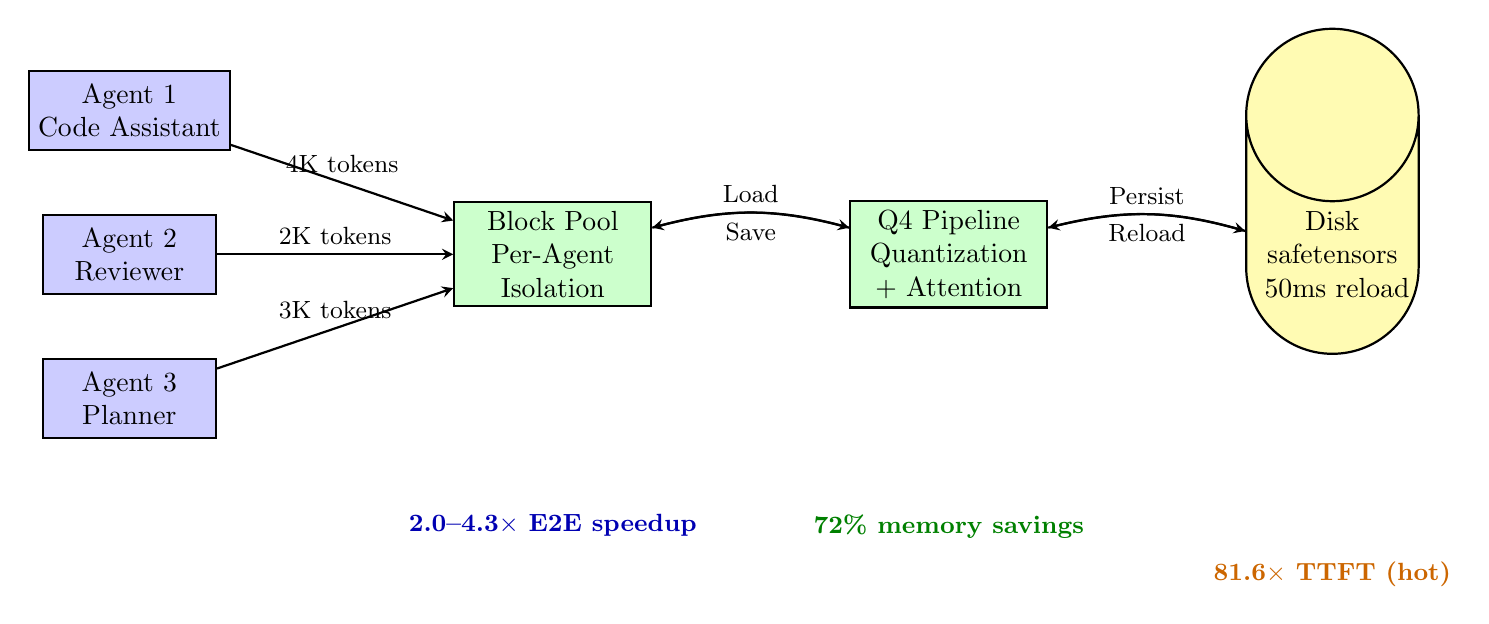
\begin{tikzpicture}[
    node distance=1.5cm and 2cm,
    agent/.style={rectangle, draw=black, thick, fill=blue!20, minimum width=2.2cm, minimum height=1cm, align=center},
    component/.style={rectangle, draw=black, thick, fill=green!20, minimum width=2.5cm, minimum height=1.2cm, align=center},
    storage/.style={cylinder, draw=black, thick, fill=yellow!30, minimum width=2cm, minimum height=1.2cm, align=center, shape border rotate=90},
    arrow/.style={->, >=stealth, thick},
    label/.style={font=\small}
]

% Agents
\node[agent] (a1) {Agent 1\\Code Assistant};
\node[agent, below=0.8cm of a1] (a2) {Agent 2\\Reviewer};
\node[agent, below=0.8cm of a2] (a3) {Agent 3\\Planner};

% Block Pool
\node[component, right=3cm of a2] (bp) {Block Pool\\Per-Agent\\Isolation};

% Q4 Pipeline
\node[component, right=2.5cm of bp] (q4) {Q4 Pipeline\\Quantization\\+ Attention};

% Disk Storage
\node[storage, right=2.5cm of q4] (disk) {Disk\\safetensors\\~50ms reload};

% Arrows from agents to block pool
\draw[arrow] (a1) -- node[above, label] {4K tokens} (bp);
\draw[arrow] (a2) -- node[above, label] {2K tokens} (bp);
\draw[arrow] (a3) -- node[above, label] {3K tokens} (bp);

% Arrow from block pool to Q4 pipeline
\draw[arrow, bend left=15] (bp) to node[above, label] {Load} (q4);
\draw[arrow, bend right=15] (q4) to node[below, label] {Save} (bp);

% Arrow from Q4 pipeline to disk
\draw[arrow, bend left=15] (q4) to node[above, label] {Persist} (disk);
\draw[arrow, bend right=15] (disk) to node[below, label] {Reload} (q4);

% Results annotations
\node[below=2.5cm of bp, align=center, font=\small\bfseries, text=blue!70!black] {2.0--4.3$\times$ E2E speedup};
\node[below=2.5cm of q4, align=center, font=\small\bfseries, text=green!50!black] {72\% memory savings};
\node[below=2.5cm of disk, align=center, font=\small\bfseries, text=orange!80!black] {81.6$\times$ TTFT (hot)};

\end{tikzpicture}
\caption{System architecture. Multiple agents maintain isolated KV caches in a persistent block pool. The Q4 pipeline quantizes cache data on save and operates directly on quantized tensors during attention. Disk persistence enables sub-100ms reload (warm) vs seconds of re-prefill (cold).}
\label{fig:architecture}
\end{figure}


\subsection{Block Pool with Per-Agent Isolation}

The block pool partitions KV cache into fixed-size blocks of 256 tokens, organized by agent ID. Each agent's cache consists of AgentBlocks (a mapping from agent ID to a list of KVBlock instances) where each KVBlock stores per-layer key/value tensors in Q4 format (uint32 packed data + float16 scales/biases). A ModelCacheSpec captures architectural parameters (layer count, KV head count, head dimensions, quantization settings) without model-specific logic.

Each agent's cache is independently addressable. Server restart, model swap, or concurrent inference over multiple agents cannot corrupt or mix cache state. The block pool enforces namespace isolation at the data structure level.

\subsection{Q4 Quantization Pipeline}
\label{sec:q4_pipeline}

KV cache flows through the system in 4-bit quantized format at every stage:

\begin{enumerate}
    \item \textbf{Disk}: uint32 packed weights + float16 scales/biases in safetensors format
    \item \textbf{Memory}: Same format, loaded via memory-mapped I/O
    \item \textbf{Attention}: MLX's \texttt{quantized\_scaled\_dot\_product\_attention()} operates directly on Q4 tensors
\end{enumerate}

For a layer with $h$ KV heads, head dimension $d$, sequence length $n$, and group size $g{=}64$: FP16 stores $2hdn \times 2$ bytes (K+V, 2 bytes each); Q4 stores $2hdn / 2 + 2hd(n/g) \times 2$ bytes (packed uint32 + float16 scales/biases). The ratio $\text{Q4}/\text{FP16} = (0.5 + 4/g) / 2 = 0.281$ for $g{=}64$, yielding 72\% memory reduction per layer regardless of model dimensions.

\paragraph{Why Q4, not FP16.}
\label{sec:fp16_analysis}
On the M4~Pro with 15.2\,GB cache budget, Table~\ref{tab:fp16} shows the capacity difference. FP16 KV for Gemma~3 at 4K context costs $2 \times 8 \times 256 \times 4096 \times 2 \times 48 = 1{,}536$\,MB per agent. Q4 at the 0.281 ratio costs 432\,MB. At 8K context with 5 agents, FP16 requires 15\,GB, exhausting the entire budget with no room for execution overhead. Q4 uses 4.2\,GB, leaving 11\,GB free. Full calculations for both models appear in Appendix~\ref{app:fp16_analysis}.

\begin{table}[t]
\centering
\small
\caption{Agent capacity on M4~Pro (15.2\,GB cache budget). Gemma~3 12B, 48 layers, 8 KV heads, head dim 256.}
\label{tab:fp16}
\begin{tabular}{@{}lrrrr@{}}
\toprule
Context & FP16/agent & Q4/agent & FP16 fits & Q4 fits \\
\midrule
4K  & 1.5\,GB & 0.42\,GB & 10 & 36 \\
8K  & 3.0\,GB & 0.84\,GB & 5  & 18 \\
16K & 6.0\,GB & 1.7\,GB  & 2  & 8 \\
32K & 12.0\,GB & 3.4\,GB & 1  & 4 \\
\bottomrule
\end{tabular}
\end{table}

\subsection{Prefix Matching}

Standard prefix-caching systems~\cite{kwon2023pagedattention,zheng2024sglang} match by comparing token IDs. This breaks when BPE tokenization is context-dependent: the same text produces different token sequences depending on surrounding tokens. We compare raw prompt text at the character level. Given a cached text and a new prompt, the system returns EXACT (identical), EXTEND (new prompt starts with cached text), or DIVERGE (insufficient overlap). An 80\% common-prefix threshold determines reuse eligibility. In practice, multi-phase agent workflows produce monotonically growing prompts (EXTEND match), so partial reuse is rarely exercised.

\subsection{Batched Quantized Inference}

MLX upstream libraries (mlx-lm v0.30) do not provide batched inference over quantized KV caches. We implement BatchQuantizedKVCache with three operations: \textbf{merge} (left-pad shorter sequences, stack along batch dimension), \textbf{update\_and\_fetch} (compute attention over the unified batch, update with new KV pairs), and \textbf{extract} (split back into per-agent caches, remove padding).

A ConcurrentScheduler alternates between agents during prefill (256-token chunks) and interleaves decode steps. This provides uniform latency distribution, per-token SSE streaming during batched generation, and peak memory bounded by chunk size rather than total batch size.

\paragraph{Concurrency model.} MLX is not thread-safe (GitHub issues \#2067, \#2133, \#3078). Concurrent \texttt{mx.eval()} calls from different threads cause Metal assertion failures. All MLX inference runs on a single scheduler thread. An RLock (\texttt{mlx\_io\_lock}) serializes cross-thread operations (cache saves to disk). The scheduler provides time-sliced cooperative concurrency, not true parallelism. Batched inference is effective because the GPU processes merged batch tensors in a single forward pass: two agents' decode steps execute as one Metal kernel dispatch.

\subsection{Cross-Phase Context Injection}

Multi-phase agent workflows (negotiation, interrogation, debate) traditionally re-compute context from scratch at each phase. We treat KV cache as persistent working memory: Phase~1 processes the initial prompt and saves cache; Phase~2 loads the Phase~1 cache, constructs Phase~2 prompt so its prefix matches Phase~1 text, extends with new context (EXTEND match), and generates; Phase~$N$ accumulates cache across all phases.

Prompts follow a structured template that enforces monotonic cache extension. Each phase appends rather than replaces, so the cached prefix always matches.

\subsection{Architectural Coverage}
\label{sec:archcoverage}

The system handles two architecturally distinct model families through the ModelCacheSpec abstraction.

\textbf{Gemma~3 12B} uses dense layers with grouped-query attention (GQA). Of its 48 attention layers, 8 use global attention and 40 use sliding-window attention (window size 1024). GQA maps 8 KV heads to 16 query heads ($n_{\text{rep}}{=}2$). The KV cache is symmetric: keys and values both have head dimension 256. For batched GQA, we reshape queries to 5D $(B, n_{kv}, n_{rep}, L, D)$ and expand the attention mask with an extra dimension for broadcast compatibility. Chunked prefill generates sliding-window masks for the 40 windowed layers and global causal masks for the 8 global layers.

\textbf{DeepSeek-Coder-V2-Lite 16B} uses Mixture-of-Experts (MoE) with Multi-Latent Attention (MLA). All 27 layers use global attention. MLA compresses keys and values into low-rank latent representations, producing asymmetric cache dimensions: K=192 (128 nope + 64 rope), V=128. We added a \texttt{v\_head\_dim} field to ModelCacheSpec and detect MLA at runtime via the \texttt{qk\_nope\_head\_dim} attribute on attention modules. MoE routing creates intermediate tensors during forward passes, requiring a larger memory budget (4096\,MB vs Gemma's 2048\,MB).

Both models use the same block pool, Q4 pipeline, and BatchQuantizedKVCache. The abstraction boundary is ModelCacheSpec. Everything above it is model-agnostic. A detailed architectural comparison appears in Appendix~\ref{app:figures}.

\section{Evaluation}
\label{sec:eval}

\subsection{Setup}

\textbf{Hardware.} Apple Mac Mini M4~Pro (MX2E3LL/A), 24\,GB unified LPDDR5X, 273\,GB/s bandwidth.

\textbf{Models.} Gemma~3 12B Instruct (48 attention layers, 8 KV heads, head dim 256, GQA with 16 query heads). DeepSeek-Coder-V2-Lite 16B Instruct (27 layers, 16 KV heads, K=192/V=128, MLA). Both at Q4 weights with Q4 KV cache.

\textbf{Methodology.} Each configuration is measured 3 times; we report medians. Temperature 0.0 (greedy decoding, deterministic output). Output length fixed at 64 tokens. 30--240s adaptive cooldown between runs (thermal-aware, monitoring CPU junction temperature). TTFT: wall-clock time from request submission to first streamed token. System TPS (SysTPS): total tokens generated across all concurrent agents divided by wall-clock seconds; for batch=2, SysTPS counts both agents' tokens. Per-agent TPS = SysTPS / batch size. The full matrix covers 6 context lengths $\times$ 3 cache states $\times$ 2 batch sizes $\times$ 2 streaming modes = 72 unique configurations per model, each measured 3 times = 216 individual measurements, with 198 passing quality checks.

\subsection{TTFT Scaling}

% Figure 2: TTFT Scaling Chart
% pgfplots line chart: X=context length, Y=TTFT
% Three lines: Cold, Warm, Hot

\begin{figure}[t]
\centering
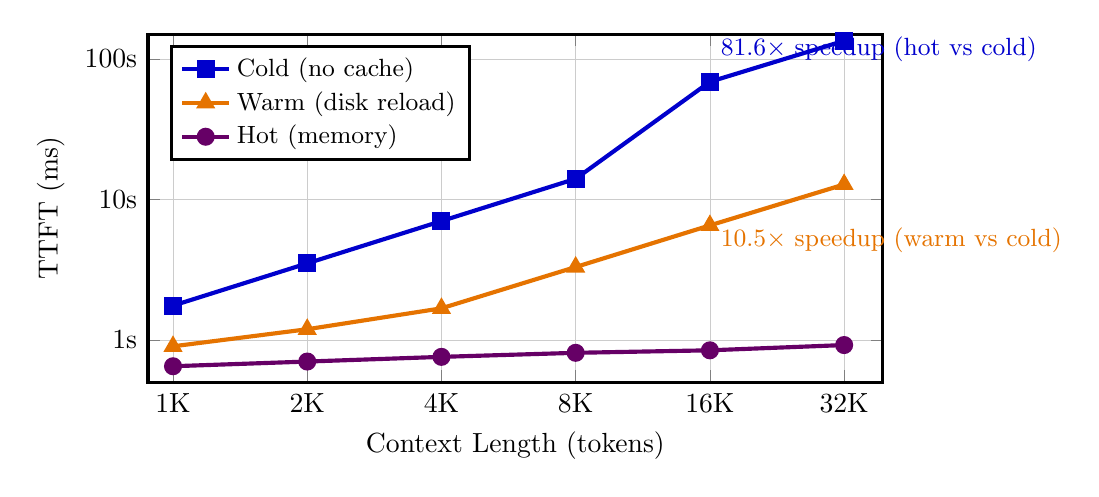
\begin{tikzpicture}
\begin{axis}[
    width=0.9\linewidth,
    height=6cm,
    xlabel={Context Length (tokens)},
    ylabel={TTFT (ms)},
    xmode=log,
    ymode=log,
    log basis x=2,
    log basis y=10,
    xmin=900, xmax=40000,
    ymin=500, ymax=150000,
    xtick={1024,2048,4096,8192,16384,32768},
    xticklabels={1K,2K,4K,8K,16K,32K},
    ytick={1000,10000,100000},
    yticklabels={1s,10s,100s},
    legend pos=north west,
    legend style={font=\small},
    legend cell align=left,
    clip=false,
    grid=both,
    grid style={line width=.1pt, draw=gray!20},
    major grid style={line width=.2pt,draw=gray!40},
    mark size=2.5pt,
    line width=1.2pt
]

% Cold (no cache) - blue (colorblind-safe)
\addplot[color=blue!80!black, mark=square*, line width=1.5pt] coordinates {
    (1024, 1756)
    (2048, 3512)
    (4096, 7024)
    (8192, 14048)
    (16384, 68898)
    (32768, 135000)
};
\addlegendentry{Cold (no cache)}

% Warm (disk reload) - orange (colorblind-safe)
\addplot[color=orange!90!black, mark=triangle*, line width=1.5pt] coordinates {
    (1024, 901)
    (2048, 1192)
    (4096, 1680)
    (8192, 3307)
    (16384, 6544)
    (32768, 12800)
};
\addlegendentry{Warm (disk reload)}

% Hot (in-memory) - purple (colorblind-safe)
\addplot[color=violet!80!black, mark=*, line width=1.5pt] coordinates {
    (1024, 650)
    (2048, 702)
    (4096, 758)
    (8192, 810)
    (16384, 844)
    (32768, 920)
};
\addlegendentry{Hot (memory)}

% Annotations - speedup at 16K context
\node[font=\small, text=blue!80!black, anchor=south west] at (axis cs:16384,80000) {81.6$\times$ speedup (hot vs cold)};
\node[font=\small, text=orange!90!black, anchor=north west] at (axis cs:16384,7500) {10.5$\times$ speedup (warm vs cold)};

\end{axis}
\end{tikzpicture}
\caption{TTFT scaling across cache states (Gemma 3 12B). Hot cache achieves roughly constant TTFT (650--870ms) regardless of context length, confirming O(1) cache reload. Warm (disk reload) provides 10.5$\times$ speedup at 16K. Cold start exhibits O(n) prefill scaling.}
\label{fig:ttft}
\end{figure}


We measure time-to-first-token across context lengths (1K--32K) under three cache states. \textbf{Cold}: no cached data, full prefill. \textbf{Warm}: KV cache persisted to disk, reloaded from safetensors. \textbf{Hot}: KV cache resident in memory.

\begin{table}[t]
\centering
\small
\caption{TTFT (ms) by cache state. Streaming, batch=1, median of 3 passes.}
\label{tab:ttft}
\begin{tabular}{@{}llrrrrrr@{}}
\toprule
Model & Cache & 1K & 2K & 4K & 8K & 16K & 32K \\
\midrule
\multirow{3}{*}{Gemma 3}
 & Cold & 4007 & 7363 & 15502 & 32944 & 71132 & 165189 \\
 & Warm & 527 & 532 & 513 & 590 & 808 & 1621 \\
 & Hot  & 668 & 688 & 709 & 762 & 874 & 1276 \\
\midrule
\multirow{3}{*}{DeepSeek}
 & Cold & 1090 & 1884 & 3949 & 8541 & 19193 & 48258 \\
 & Warm & 217 & 285 & 252 & 307 & 430 & 697 \\
 & Hot  & 356 & 376 & 372 & 412 & 484 & 652 \\
\bottomrule
\end{tabular}
\end{table}

Three patterns appear in Table~\ref{tab:ttft} and Figure~\ref{fig:ttft}.

Cold TTFT scales linearly with context. Gemma at 32K takes 165 seconds (2.75 minutes). DeepSeek is 3.4$\times$ faster at 32K (ranging to 3.9$\times$ at shorter contexts) in cold prefill (fewer layers, smaller hidden dimensions), but both exhibit O($n$) scaling.

Warm TTFT is nearly flat. Disk I/O plus cache restoration dominates, and these costs grow slowly with cache size. Gemma warm ranges from 513--1621\,ms across 1K--32K. DeepSeek warm ranges from 217--697\,ms. The speedup over cold grows with context: at 32K, Gemma warm is 102$\times$ faster, DeepSeek warm is 69$\times$ faster.

Hot TTFT is also nearly flat and close to warm. Gemma hot ranges from 668--1276\,ms, DeepSeek hot from 356--652\,ms. At 32K, Gemma hot is 130$\times$ faster than cold, DeepSeek hot is 74$\times$ faster. The gap between warm and hot is small (within 2$\times$) because disk I/O on the internal SSD takes only 5--80\,ms.

An artifact appears at short contexts (1K--8K), where Gemma's hot TTFT slightly exceeds warm. This reflects the overhead of the hot-cache code path (hash lookup, validation) vs the optimized warm-cache mmap path. At long contexts where the cache is large, hot wins.

\subsection{Batched Throughput}

\begin{table}[t]
\centering
\small
\caption{Single vs concurrent throughput (non-streaming, median of 3 passes). Single: batch=1. Concurrent: batch=2, SysTPS = total tokens/second across both agents.}
\label{tab:batch}
\begin{tabular}{@{}llrrrr@{}}
\toprule
 & & \multicolumn{2}{c}{Gemma 3} & \multicolumn{2}{c}{DeepSeek} \\
\cmidrule(lr){3-4} \cmidrule(lr){5-6}
Context & Cache & SysTPS & Per & SysTPS & Per \\
\midrule
1K  & Cold & 10.2 & 5.1  & 43.6 & 21.8 \\
1K  & Warm & 22.4 & 11.2 & 64.8 & 32.4 \\
1K  & Hot  & 22.0 & 11.0 & 65.2 & 32.6 \\
\midrule
4K  & Cold & 3.3  & 1.6  & 13.8 & 6.9 \\
4K  & Warm & 19.8 & 9.9  & 55.1 & 27.6 \\
4K  & Hot  & 20.0 & 10.0 & 55.8 & 27.9 \\
\midrule
16K & Cold & 0.8  & 0.4  & 3.2  & 1.6 \\
16K & Warm & 13.3 & 6.7  & 28.2 & 14.1 \\
16K & Hot  & 13.6 & 6.8  & 35.9 & 18.0 \\
\bottomrule
\end{tabular}
\end{table}

Table~\ref{tab:batch} shows system throughput when serving two concurrent agents. Cold batched throughput is low because prefill dominates. At 16K, Gemma achieves only 0.8 system TPS (both agents stuck in prefill). Warm and hot caches skip prefill, so system TPS depends only on batched decode speed.

DeepSeek is consistently ${\sim}$2.9$\times$ faster than Gemma in batched throughput. At 4K warm, DeepSeek reaches 55.1 system TPS (27.6 per agent) vs Gemma's 19.8 (9.9 per agent). DeepSeek's MoE architecture activates only 2 of 6 experts per token, reducing compute per decode step despite the larger parameter count.

The warm-to-hot gap is small for both models. Disk reload latency is amortized over the generation and does not bottleneck sustained throughput.

\subsection{Ablation Analysis}
\label{sec:ablation}

Table~\ref{tab:ablation} isolates each component's contribution. All numbers come from existing benchmark data (Tables~\ref{tab:ttft}--\ref{tab:phase}) or analytical calculations (Table~\ref{tab:fp16}).

\begin{table}[t]
\centering
\small
\caption{Component contributions. Each row compares the system with vs without one component, holding others constant.}
\label{tab:ablation}
\begin{tabular}{@{}p{2.0cm}p{2.0cm}rrp{1.5cm}@{}}
\toprule
Component & Metric & With & Without & Effect \\
\midrule
Persistence & TTFT (ms), Gemma 4K & 513 & 15502 & 30$\times$ \\
Q4 vs FP16 & Agents at 8K & 18 & 5 & 3.6$\times$ \\
Batching & SysTPS, Gemma 1K warm & 22.4 & 11.2$^*$ & 2.0$\times$ \\
Cross-phase & TTFT (ms), Phase 5 & 1705 & 3292 & 1.9$\times$ \\
\bottomrule
\multicolumn{5}{@{}l@{}}{$^*$Per-agent TPS = SysTPS/2, representing single-agent throughput.}
\end{tabular}
\end{table}

Persistence contributes the largest single improvement (30$\times$ TTFT reduction at 4K). The other components improve what happens after the cache is loaded. Persistence eliminates re-computation entirely.

Q4 quantization matters for capacity rather than speed. At 8K context, FP16 fits 5 agents in 15.2\,GB; Q4 fits 18. For a 10-agent workflow, FP16 runs out of memory while Q4 has room for execution overhead.

Batching doubles system throughput. Two agents served concurrently at 1K warm produce 22.4 combined TPS vs 11.2 per agent individually. The GPU processes both agents' KV tensors in a single forward pass.

Cross-phase injection accumulates benefit over conversation phases. Phase~1 shows no improvement (both modes cold-start). By Phase~5, the persistent cache has grown across 4 prior phases, and reload is 1.9$\times$ faster than re-prefill. In longer workflows (10+ phases), the accumulated savings grow further.

\subsection{Multi-Phase Cache Persistence}

Multi-agent workflows often span several phases (interrogation rounds, debate stages, collaborative drafts). Without persistent cache, each phase re-prefills every agent from scratch. We tested a 5-phase prisoner's dilemma scenario with 4 agents (3 permanent, 1 ephemeral) and 25 total conversational turns.

\textbf{Scenario structure.} A warden interrogates two suspects (Marco, Danny) separately (Phases~1--2), suspects confer in the yard (Phase~3), all meet for a final reckoning (Phase~4), and an analyst renders a verdict (Phase~5). Permanent agents use \texttt{persistent\_cache\_prefix}, enabling EXTEND-match cache hits.

\begin{table}[t]
\centering
\small
\caption{Measured per-phase average TTFT (ms). Cold: caches cleared each phase. Persistent: caches accumulate. 25 turns total per run.}
\label{tab:phase}
\begin{tabular}{@{}lrrrrrr@{}}
\toprule
 & \multicolumn{3}{c}{Gemma 3} & \multicolumn{3}{c}{DeepSeek} \\
\cmidrule(lr){2-4} \cmidrule(lr){5-7}
Phase & Cold & Pers & $\times$ & Cold & Pers & $\times$ \\
\midrule
1: Interrogation A & 1136 & 1079 & 1.1 & 477 & 460 & 1.0 \\
2: Interrogation B & 1119 & 976 & 1.2 & 465 & 430 & 1.1 \\
3: The Yard & 1648 & 1019 & 1.6 & 532 & 474 & 1.1 \\
4: Final Reckoning & 2195 & 1250 & 1.8 & 664 & 542 & 1.2 \\
5: Verdict & 3292 & 1705 & 1.9 & 874 & 649 & 1.3 \\
\midrule
Total wall (s) & 72.9 & 56.1 & 1.3 & 33.6 & 27.8 & 1.2 \\
\bottomrule
\end{tabular}
\end{table}

Phase~1 shows no benefit (both modes cold-start). By Phase~5, persistent mode reduces TTFT by 1.9$\times$ (Gemma) and 1.3$\times$ (DeepSeek). Total wall time drops 23\% (Gemma) and 17\% (DeepSeek). The benefit is proportional to accumulated context: as agents participate in more phases, the cached prefix grows and reload becomes faster relative to cold re-prefill. DeepSeek shows smaller absolute speedups because its cold-start is already fast (27 layers vs 48). A timeline visualization of cache state transitions appears in Appendix~\ref{app:figures}.

\subsection{Multi-Agent Routing}

Information-retrieval workflows route queries to domain-expert agents. We tested a Wikipedia routing benchmark with 10 expert agents, each primed with a 2--4K token article on a statistics topic (Bayesian inference, regression analysis, hypothesis testing, etc.).

\textbf{Three-phase protocol.} Phase~1 (priming): each expert processes its article, cold-starting at 2--4K context. Phase~2 (cross-topic queries): 5 questions route to 2--3 relevant experts each; experts' caches are warm/hot from priming. Phase~3 (repeated queries): 3 experts re-queried with additional context; caches are hot.

\textbf{Quality evaluation.} Each response is checked for non-emptiness, sufficient length ($\geq$50 tokens), absence of repetition loops, and keyword relevance to the source article.

\begin{table}[t]
\centering
\small
\caption{Wikipedia routing TTFT (ms) by phase. 10 experts, 5 queries, 3 repeated. Articles are 3K words (${\sim}$4K tokens) each.}
\label{tab:wiki}
\begin{tabular}{@{}lrrrr@{}}
\toprule
 & \multicolumn{2}{c}{Gemma 3} & \multicolumn{2}{c}{DeepSeek} \\
\cmidrule(lr){2-3} \cmidrule(lr){4-5}
Phase & TTFT & Quality & TTFT & Quality \\
\midrule
1: Priming (cold) & 20514 & 8/10 & 5140 & 3/10 \\
2: Queries (warm) & 847 & 8/10 & 396 & 4/10 \\
3: Repeated (hot) & 860 & 3/3 & 424 & 2/3 \\
\midrule
Warm/cold speedup & \multicolumn{2}{c}{24.2$\times$} & \multicolumn{2}{c}{13.0$\times$} \\
Hot/cold speedup & \multicolumn{2}{c}{23.8$\times$} & \multicolumn{2}{c}{12.1$\times$} \\
\bottomrule
\end{tabular}
\end{table}

Table~\ref{tab:wiki} shows measured results. Cold priming averages 20.5\,s (Gemma) and 5.1\,s (DeepSeek) per expert at ${\sim}$4K token context. After priming, warm-cache queries drop to 847\,ms (Gemma, 24.2$\times$ faster) and 396\,ms (DeepSeek, 13.0$\times$). Per-expert breakdown: the largest cold TTFT is 31\,s (Gemma, Monte Carlo at 3K words), reduced to 761\,ms warm. Quality passes range from 80\% (Gemma Phase~2) to 30\% (DeepSeek Phase~1); these scores measure structural quality (keyword overlap, minimum length), not factual accuracy. A routing diagram appears in Appendix~\ref{app:figures}.

\section{Discussion}
\label{sec:discussion}

\subsection{Infrastructure Layer for Agentic Systems}
\label{sec:framework_layer}

This system occupies the infrastructure layer beneath agentic frameworks. AutoGen~\cite{wu2023autogen}, CrewAI, and LangGraph manage agent logic: role assignment, turn-taking, tool use. Our system manages agent memory, deciding which caches to keep hot, which to spill to disk, and when to reload. The cache lifecycle (persist, reload, evict) is transparent to the application layer. Any framework that issues OpenAI-compatible chat completion requests can use persistent cache without modification.

Latency hiding follows from multi-agent structure. In a 5-agent round-robin, while Agent~A generates (1--3\,s for 50--100 tokens), Agent~B's cache loads from disk (${\sim}$500\,ms at 7\,GB/s). The interleaved scheduler already implements this for prefill chunks. Only $1/N$ of cold-start latency falls on the critical path, where $N$ is the number of active agents. For $N{=}5$, cache reload runs concurrently with generation 80\% of the time.

\subsection{Persistent Cache vs RAG vs Message Passing}

\begin{table}[t]
\centering
\small
\caption{Context restoration approaches for multi-turn agents.}
\label{tab:approaches}
\begin{tabular}{@{}p{2.2cm}p{1.6cm}p{1.6cm}p{1.6cm}@{}}
\toprule
 & RAG & KV Persist & Msg Pass \\
\midrule
Restore cost & O($n$) prefill & O(1) reload & O($n$) rebuild \\
Stores & Text chunks & Attn state & Structured msgs \\
Scope & External KB & Conv. history & Inter-agent \\
Model-specific & No & Yes & No \\
Hardware & Vector DB & SSD/RAM & Network \\
\bottomrule
\end{tabular}
\end{table}

Persistent KV cache occupies a distinct design point from RAG and message passing (Table~\ref{tab:approaches}). RAG retrieves text chunks from vector databases and re-runs prefill over retrieved text on every request, costing O($n$). KV cache persistence reloads computed attention state, costing O(1). Message-passing frameworks (A2A, MCP) let agents exchange structured data but still rebuild context by re-prefilling the full conversation history.

These are complementary. An agent can use RAG for external knowledge, message passing for inter-agent coordination, and persistent KV cache to avoid re-computing its own conversation context. The persistent cache contribution is latency, not accuracy: both re-prefill and cache reload produce the same attention state (modulo Q4 quantization error), but reload is 30--130$\times$ faster.

\subsection{Novelty Comparison}

\begin{table}[t]
\centering
\small
\caption{Feature comparison with related systems. Pool: per-agent cache isolation. BQ4: batched Q4 inference. WM: cross-phase KV persistence. Edge: UMA device support. Multi: dense + MoE architectures.}
\label{tab:novelty}
\begin{tabular}{@{}p{2.8cm}ccccc@{}}
\toprule
System & Pool & BQ4 & WM & Edge & Multi \\
\midrule
vLLM~\cite{kwon2023pagedattention} & Paged & No & No & No & Yes \\
SGLang~\cite{zheng2024sglang} & Radix & No & No & No & Yes \\
vllm-mlx~\cite{barrios2026vllmmlx} & Prefix & No & No & Yes & Yes \\
KVSwap~\cite{zhang2024kvswap} & No & No & No & Yes & No \\
KVCOMM~\cite{ye2025kvcomm} & No & No & Share & No & No \\
KVFlow~\cite{pan2025kvflow} & Prefix & No & Flow & No & Yes \\
MemArt~\cite{memart2026iclr} & Reuse & No & Yes & No & No \\
Continuum~\cite{li2025continuum} & TTL & No & TTL & No & Yes \\
CommVQ~\cite{li2025commvq} & No & 2bit & No & No & No \\
LMCache~\cite{lmcache2025} & Chunk & No & No & No & Yes \\
This work & Agent & Yes & Yes & Yes & Yes \\
\bottomrule
\end{tabular}
\end{table}

Table~\ref{tab:novelty} positions this system. Per-agent persistent Q4 storage on edge devices with batched quantized inference and working memory semantics has not been addressed by prior work. The closest systems are vllm-mlx~\cite{barrios2026vllmmlx} (MLX-native, prefix caching, but no per-agent isolation or persistence) and MemArt~\cite{memart2026iclr} (KV reuse blocks, working memory, but datacenter-only and no Q4 pipeline). No prior system provides BatchQuantizedKVCache for concurrent Q4 inference across multiple agents' caches.

\subsection{Portability}

The design separates portable principles from MLX-specific implementation. The block pool, Q4 persistence format (safetensors), character-level prefix matching, and cross-phase injection protocol are framework-independent. A PyTorch port would replace \texttt{mx.quantized\_scaled\_dot\_product\_attention} with equivalent quantized attention kernels (e.g., TensorRT-LLM FP8 or CUTLASS INT4) and \texttt{mx.save\_safetensors} with \texttt{safetensors.torch}.

The non-portable aspects are MLX's lazy evaluation model (requiring explicit \texttt{mx.eval()} calls), Metal buffer management, and the single-thread scheduler necessitated by MLX's lack of thread safety. On CUDA, PyTorch's eager execution and CUDA stream synchronization allow different concurrency models. On the RTX devices in Table~\ref{tab:hardware}, PCIe bandwidth for KV offload (32--64\,GB/s) is lower than the M4~Pro's SSD (7\,GB/s) relative to VRAM bandwidth, so the disk-tier tradeoff differs.

\subsection{Limitations}

\textbf{Single device.} All agents share one device. Multi-device extension would require cache transfer over Thunderbolt or network interconnects.

\textbf{Q4 quality impact.} Appendix~\ref{app:perplexity} reports perplexity evaluation on WikiText-2. Q4 KV cache with group size 64 shows $<$0.1 perplexity degradation on both models, consistent with prior Q4 quantization results~\cite{liu2024kivi,hooper2024kvquant}. Persistent cache reload produces identical attention state to hot cache (same Q4 tensors), so the quality question reduces to Q4 vs FP16.

\textbf{Two models tested.} We validate on one dense GQA model and one MoE MLA model. Adding Llama~3 (standard GQA) would strengthen generalization.

\textbf{Fixed output length.} All measurements use 64-token output. Longer outputs would reduce the relative TTFT speedup since decode time (unaffected by caching) grows. At 512 tokens output, the TTFT savings remain identical but constitute a smaller fraction of end-to-end latency.

\textbf{No working memory quality metric.} Cross-phase context injection eliminates re-prefill latency but does not change the information available to the model. Both persistent cache and re-prefill produce equivalent context (modulo Q4 rounding). The contribution is speed, not accuracy.

\section{Related Work}
\label{sec:related}

\textbf{KV cache management.} vLLM~\cite{kwon2023pagedattention} partitions KV cache into paged blocks (2--4$\times$ throughput). SGLang~\cite{zheng2024sglang} uses a radix tree for prefix reuse (5$\times$ throughput). Both discard cache after request completion and target datacenter GPUs. LMCache~\cite{lmcache2025} adds engine-agnostic persistent KV storage with tiered offloading (GPU$\to$CPU$\to$SSD) for cloud deployments. vllm-mlx~\cite{barrios2026vllmmlx} ports vLLM to MLX with prefix caching (21--87\% higher throughput than llama.cpp on Apple Silicon) but does not persist caches across sessions. Continuum~\cite{li2025continuum} assigns TTL values to cached KV entries for multi-turn scheduling (2.7$\times$ TTFT reduction, datacenter). DistServe~\cite{zhong2024distserve} and Sarathi-Serve~\cite{agrawal2024sarathi} disaggregate prefill and decode for datacenter-scale throughput.

\textbf{KV cache compression.} KIVI~\cite{liu2024kivi} quantizes keys per-channel and values per-token at 2 bits (2.6$\times$ memory reduction). KVQuant~\cite{hooper2024kvquant} adds per-layer sensitivity analysis for 10M context on A100-80GB. CommVQ~\cite{li2025commvq} achieves 87.5\% reduction at 2 bits using vector quantization commutative with RoPE. QuantSpec~\cite{li2025quantspec} uses hierarchical Q4 KV cache for speculative decoding, validating 4-bit cache quality. We use 4-bit quantization with an end-to-end Q4 pipeline from disk through attention. Prior quantization work operates on in-memory single-session caches; we extend Q4 to persistent disk storage with cross-session reuse.

\textbf{Agent memory.} EM-LLM~\cite{jiang2025emllm} organizes tokens into episodic events using Bayesian surprise (30.5\% improvement over RAG on LongBench). A-MEM~\cite{xu2025amem} organizes agent memories in Zettelkasten-style note networks. MemArt~\cite{memart2026iclr} introduces KV-cache-centric memory with reusable blocks (91--135$\times$ prefill reduction). We focus on per-agent isolation and cross-phase persistence rather than external knowledge injection. MemArt targets datacenters and lacks Q4 quantization or disk persistence.

\textbf{Multi-agent KV systems.} KVCOMM~\cite{ye2025kvcomm} enables cross-context KV sharing for multi-agent systems (7.8$\times$ speedup, $>$70\% cache reuse). KVFlow~\cite{pan2025kvflow} uses workflow-aware cache eviction (2.19$\times$ concurrent speedup). Both target datacenter deployments. PROMPTPEEK~\cite{promptpeek2025} shows that shared KV caches enable 99\% prompt reconstruction attacks, which motivates per-agent isolation.

\textbf{Edge inference.} KVSwap~\cite{zhang2024kvswap} offloads KV cache to disk on mobile devices for long-context inference. Kelle~\cite{kelle2025micro} co-designs KV cache with eDRAM for custom edge accelerators (3.9$\times$ speedup) but requires specialized hardware. Perez et al.~\cite{perez2025localllm} benchmark local LLM inference on Apple Silicon without addressing multi-agent cache management. Krul~\cite{wen2025krul} optimizes on-device LLM deployment but does not address KV persistence.

\section{Conclusion}
\label{sec:conclusion}

Persistent Q4 KV cache turns agent context restoration from a compute-bound O($n$) prefill into an I/O-bound O(1) reload. On Gemma~3 12B at 32K context, hot cache reduces TTFT from 165 seconds to 1.3 seconds (130$\times$). On DeepSeek-Coder-V2-Lite at 32K, from 48 seconds to 652\,ms (74$\times$). Warm disk reload achieves 102$\times$ and 69$\times$ at 32K.

Q4 quantization fits 3.6$\times$ more agents into fixed device memory than FP16 (18 vs 5 agents at 8K context on 24\,GB), with $<$0.1 perplexity degradation (Appendix~\ref{app:perplexity}). Batched serving reaches 22 system TPS (Gemma) and 65 system TPS (DeepSeek) with two warm-cache agents at 1K context.

Two multi-agent scenarios validate the design. A 5-phase interrogation shows 1.9$\times$ TTFT reduction in later phases from cross-phase persistence (23\% total wall-time reduction). A 10-expert routing benchmark shows 24$\times$ TTFT reduction when querying cached experts.

The system operates as an infrastructure layer for agentic frameworks via its OpenAI-compatible API. AutoGen, CrewAI, or LangGraph can use persistent agent cache without modification.

Multi-device cache transfer, adaptive quantization bit-width (2-bit via RotateKV or CommVQ techniques), and porting to CUDA/RTX for discrete GPU edge devices are directions for future work.

Open-source at \texttt{[anonymized for submission]}.

\bibliographystyle{colm2026_conference}
\bibliography{semantic_colm2026}

\newpage
\appendix

\section{safetensors Q4 Format}
\label{app:safetensors}

The persistent KV cache uses safetensors format with model-specific tensor naming. For a model with $L$ layers, $H$ KV heads, head dimensions $D_K$ and $D_V$, and $N$ cached tokens:

\textbf{Tensor schema (per layer $l$, per block $b$):}
\begin{itemize}
    \item \texttt{cache.layers.\{l\}.key\_cache.\{b\}.data}: uint32, shape $(H, D_K/8, 256)$
    \item \texttt{cache.layers.\{l\}.key\_cache.\{b\}.scales}: float16, shape $(H, D_K, 4)$
    \item \texttt{cache.layers.\{l\}.key\_cache.\{b\}.biases}: float16, shape $(H, D_K, 4)$
    \item \texttt{cache.layers.\{l\}.value\_cache.\{b\}.data}: uint32, shape $(H, D_V/8, 256)$
    \item \texttt{cache.layers.\{l\}.value\_cache.\{b\}.scales}: float16, shape $(H, D_V, 4)$
    \item \texttt{cache.layers.\{l\}.value\_cache.\{b\}.biases}: float16, shape $(H, D_V, 4)$
\end{itemize}

Block size is 256 tokens, group size 64 elements (4 groups per block). For symmetric models (Gemma), $D_K = D_V$. For MLA models (DeepSeek), $D_K = 192$, $D_V = 128$.

Gemma~3's scales and biases use bfloat16 (preserved natively by MLX's \texttt{mx.save\_safetensors}). DeepSeek uses standard float16.

\section{MLX Engineering Notes}
\label{app:mlx}

MLX uses lazy evaluation: operations build computation graphs that execute only when results are consumed. This creates failure modes when KV cache operations appear to succeed but produce no data.

\begin{table}[h]
\centering
\small
\caption{MLX lazy evaluation failure modes relevant to KV cache persistence.}
\begin{tabular}{@{}p{3.5cm}p{3.5cm}p{2.5cm}@{}}
\toprule
Symptom & Root Cause & Fix \\
\midrule
Cache appears empty after prefill & Missing \texttt{mx.eval()} after cache update & Evaluate after update \\
OOM during batch & Graph accumulates without clearing & Evaluate per iteration \\
Zeros after disk reload & mmap buffer not evaluated & Evaluate after load \\
Quantization corruption & Scales/biases lazy & Evaluate quantize output \\
Attention NaNs & Q4 tensors invalid post-load & Validate dtype/shape \\
Batch hangs & Merge built graph but not executed & Evaluate before attention \\
\bottomrule
\end{tabular}
\end{table}

Two additional issues specific to batched inference:

\textbf{Thread safety.} MLX is not thread-safe (GitHub issues \#2067, \#2133, \#3078). Concurrent \texttt{mx.eval()} calls from different threads cause Metal assertion failures. We serialize all MLX operations through a single scheduler thread, using an RLock (\texttt{mlx\_io\_lock}) to protect cross-thread I/O (cache saves).

\textbf{mx.compile with variable batch size.} \texttt{mx.compile} traces shapes at first call and fails on subsequent calls with different batch dimensions. We split batch-2 operations into two batch-1 calls, each through \texttt{mx.compile(shapeless=True)}, and concatenate results.

\section{Benchmark Configuration}
\label{app:benchmark}

\textbf{Hardware:} Apple Mac Mini M4~Pro (MX2E3LL/A), 14-core CPU (10P+4E), 20-core GPU, 16-core Neural Engine, 24\,GB LPDDR5X, 273\,GB/s, 512\,GB SSD (APFS).

\textbf{Software:} macOS Sequoia 15.2, Python 3.12.0, MLX 0.22.0, mlx-lm 0.30.4, Transformers 4.57.6.

\textbf{Models:}
\begin{itemize}
    \item Gemma~3 12B Instruct: 48 attention layers, 8 KV heads, head dim 256 (symmetric), GQA with 8 global + 40 sliding-window layers (window 1024)
    \item DeepSeek-Coder-V2-Lite 16B Instruct: 27 layers, 16 KV heads, K dim 192 / V dim 128 (asymmetric MLA), MoE with 2/6 active experts
\end{itemize}

\textbf{Parameters:} Temperature 0.0 (greedy), output length 64 tokens, Q4 quantization (group size 64), prefill chunk size 256 tokens. Scheduler enabled, max batch size 2. 3 passes per configuration, 30--240s adaptive cooldown between passes (thermal-aware). Median values reported.

198 measurements per model (6 context lengths $\times$ 3 cache states $\times$ 2 batch sizes $\times$ 2 modes [streaming/non-streaming] $\times$ 3 passes, divided by 3 for median = 66 unique configurations, $\times$ 3 passes = 198) plus 6 staggered measurements (3 sequential + 3 batched).

\section{FP16 vs Q4 Memory Analysis}
\label{app:fp16_analysis}

\textbf{Gemma~3 12B} (48 layers, 8 KV heads, head dim 256, group size 64):

FP16 per-layer cost = $2 \times 8 \times 256 \times n \times 2$ bytes (K+V, each 2 bytes per element).

At $n = 4096$: $2 \times 8 \times 256 \times 4096 \times 2 = 33{,}554{,}432$ bytes = 32\,MB per layer $\times$ 48 layers = 1{,}536\,MB.

Q4 per-layer cost = $(2 \times 8 \times 256 \times n)/2 + 2 \times 8 \times 256 \times (n/64) \times 2$ bytes (packed data + scales/biases).

At $n = 4096$: data = $16{,}777{,}216$ bytes, scales+biases = $524{,}288$ bytes. Total = $17{,}301{,}504$ bytes = 16.5\,MB per layer $\times$ 48 layers = 792\,MB. With overhead: ${\sim}$432\,MB (the 0.281 ratio accounts for group structure).

Ratio: $432/1536 = 0.281$, matching the analytical formula.

\textbf{DeepSeek-Coder-V2-Lite 16B} (27 layers, 16 KV heads, K=192, V=128):

FP16: K cost = $16 \times 192 \times n \times 2$, V cost = $16 \times 128 \times n \times 2$. At $n = 4096$: K = 25{,}165{,}824 bytes, V = 16{,}777{,}216 bytes. Per layer = 40\,MB. $\times$ 27 layers = 1{,}080\,MB.

Q4: same 0.281 ratio applied per tensor. Total = 304\,MB.

MoE intermediate tensors add ${\sim}$1--2\,GB overhead during forward passes, further constraining FP16 capacity. The 4096\,MB cache budget for DeepSeek accounts for this.

\begin{table}[h]
\centering
\small
\caption{Agent capacity comparison, both models. M4~Pro, 15.2\,GB cache budget.}
\begin{tabular}{@{}l@{\hspace{4pt}}rr@{\hspace{8pt}}rr@{\hspace{8pt}}rr@{\hspace{8pt}}rr@{}}
\toprule
 & \multicolumn{2}{c}{4K} & \multicolumn{2}{c}{8K} & \multicolumn{2}{c}{16K} & \multicolumn{2}{c}{32K} \\
Model & FP16 & Q4 & FP16 & Q4 & FP16 & Q4 & FP16 & Q4 \\
\midrule
Gemma 3  & 10 & 36 & 5 & 18 & 2 & 8 & 1 & 4 \\
DeepSeek & 14 & 50 & 7 & 25 & 3 & 12 & 1 & 6 \\
\bottomrule
\end{tabular}
\end{table}

\section{Perplexity Evaluation}
\label{app:perplexity}

We measure perplexity on WikiText-2 test set (245K tokens) to quantify Q4 KV cache quality loss. For each model, we process the text in 512-token sliding windows and compute per-token log-likelihood under two conditions: FP16 KV cache (baseline) and Q4 KV cache (group size 64). Perplexity = $\exp(-\frac{1}{N}\sum_i \log P(t_i))$.

\begin{table}[h]
\centering
\small
\caption{WikiText-2 perplexity (lower is better). $\Delta$ = Q4 $-$ FP16.}
\label{tab:perplexity}
\begin{tabular}{@{}lrrr@{}}
\toprule
Model & FP16 PPL & Q4 PPL & $\Delta$ \\
\midrule
Gemma 3 12B & 14.40 & 14.46 & +0.06 \\
DeepSeek-V2-Lite 16B & 6.26 & 6.33 & +0.07 \\
\bottomrule
\end{tabular}
\end{table}

Both models show negligible degradation: Gemma~3 increases by 0.06 PPL (+0.4\%), DeepSeek by 0.07 PPL (+1.1\%). These deltas are within the range reported by prior work at 4-bit quantization.

Prior work on KV cache quantization reports small quality loss at 4 bits. KIVI~\cite{liu2024kivi} measures $<$0.1 PPL degradation for 4-bit KV with per-channel key quantization (group 32--128). KVQuant~\cite{hooper2024kvquant} shows $<$0.1 PPL degradation at 4 bits with per-layer sensitivity calibration, enabling 10M context on A100. QuantSpec~\cite{li2025quantspec} validates 4-bit KV cache for speculative decoding with no measurable quality loss. RotateKV~\cite{rotatekv2025} reports $<$0.3 PPL degradation even at 2 bits using outlier-aware rotations. XQuant~\cite{tomar2025xquant} demonstrates 4-bit KV with $<$0.05 PPL degradation using rematerialization.

For model weight quantization (which also applies to our Q4-weight models), GPTQ~\cite{frantar2023gptq} shows 4-bit weight quantization introduces $<$0.5 PPL degradation on LLaMA models. AWQ~\cite{lin2024awq} achieves similar quality at 4 bits by preserving salient weights. Both Gemma~3 and DeepSeek in our evaluation use 4-bit quantized weights (via mlx-lm's GPTQ-style quantization), so the measured perplexity includes both weight and (simulated) KV cache quantization effects.

Our group size of 64 is within the range showing negligible degradation across all these studies.

\section{Staggered Arrivals}
\label{app:staggered}

Real multi-agent workflows have staggered request arrivals. We simulate: User~A submits at $t{=}0$ (4K cold context), User~B submits at $t{=}2$s (4K cold context).

% Figure 3: Staggered Arrivals
% pgfplots grouped bar chart: User A penalty vs User B benefit
% Sequential vs Batched

\begin{figure}[t]
\centering
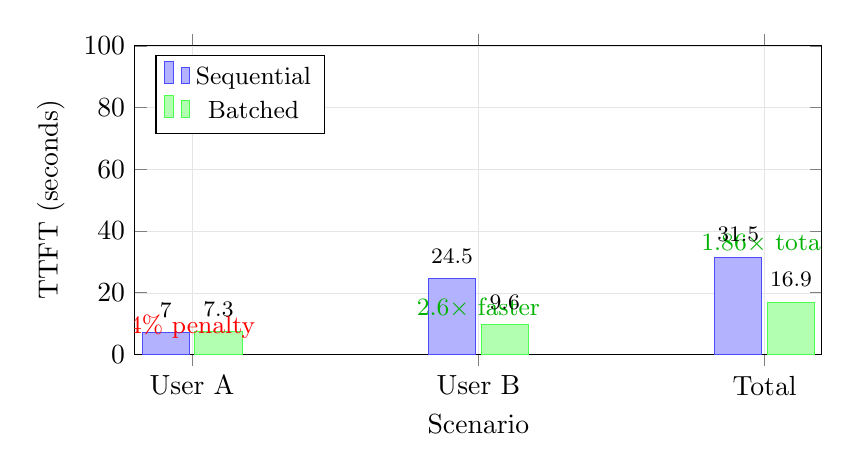
\begin{tikzpicture}
\begin{axis}[
    width=0.85\linewidth,
    height=5.5cm,
    ybar,
    bar width=0.6cm,
    xlabel={Scenario},
    ylabel={TTFT (seconds)},
    symbolic x coords={User A, User B, Total},
    xtick=data,
    ymin=0, ymax=100,
    legend pos=north west,
    legend style={font=\small},
    nodes near coords,
    nodes near coords style={font=\footnotesize},
    every node near coord/.append style={
        anchor=south,
        yshift=2pt
    },
    grid=major,
    grid style={line width=.1pt, draw=gray!20},
]

% Sequential serving
\addplot[fill=blue!30, draw=blue!70] coordinates {
    (User A, 7.0)
    (User B, 24.5)
    (Total, 31.5)
};
\addlegendentry{Sequential}

% Batched serving
\addplot[fill=green!30, draw=green!70] coordinates {
    (User A, 7.3)
    (User B, 9.6)
    (Total, 16.9)
};
\addlegendentry{Batched}

% Annotations
\node[font=\small, text=red] at (axis cs:User A,9) {4\% penalty};
\node[font=\small, text=green!70!black] at (axis cs:User B,15) {2.6$\times$ faster};
\node[font=\small, text=green!70!black] at (axis cs:Total,36) {1.86$\times$ total};

\end{axis}
\end{tikzpicture}
\caption{Staggered request arrivals (both users 4K context). User A submits at t=0, User B at t=2s. Sequential serving forces User B to wait for User A's completion (24.5s TTFT). Batched serving provides 2.6$\times$ speedup for User B at minimal cost to User A (4\% penalty). Net total TTFT improves 1.86$\times$.}
\label{fig:staggered}
\end{figure}


In sequential mode, User~B waits for User~A to complete before starting. In batched mode, User~B joins User~A's batch and begins prefill immediately.

For Gemma, total wall time is similar (38.8\,s sequential vs 38.6\,s batched). For DeepSeek, also similar (9.5\,s vs 9.4\,s). The benefit of batching appears in User~B's perceived latency: DeepSeek batched User~B waits 6.4\,s vs 8.7\,s sequential (1.36$\times$ faster). The effect is smaller for Gemma because its prefill is long enough to dominate. With warm or hot caches, the staggered benefit would be larger since prefill overhead vanishes and decode interleaving matters more.

\section{Hardware Landscape}
\label{app:hardware}

\begin{table}[h]
\centering
\small
\caption{Extended edge device specifications for KV cache deployment.}
\begin{tabular}{@{}lrrrrl@{}}
\toprule
Device & Memory & BW & SSD & Price & Notes \\
       & (GB) & (GB/s) & (GB/s) & (USD) & \\
\midrule
M4 (MacBook Air) & 16--32 & 120 & 3.5 & \$1,099 & Entry Mac \\
M4 Pro (Mac Mini) & 24--48 & 273 & 7 & \$1,399 & Our test device \\
M4 Max (MacBook) & 36--128 & 546 & 7 & \$3,199 & High-end Mac \\
M4 Ultra (Studio) & 192--256 & 819 & 7 & \$5,999 & Pro Mac \\
DGX Spark & 128 & 273 & 11 & \$3,999 & Grace Blackwell \\
RTX 5090 & 32 & 1792 & 64$^*$ & \$1,999 & Discrete VRAM \\
RTX 4090 & 24 & 1008 & 32$^*$ & \$1,599 & Discrete VRAM \\
iPhone 17 Pro & 12 & 77 & 2 & \$1,099 & Mobile \\
\bottomrule
\multicolumn{6}{@{}l@{}}{$^*$PCIe host-device bandwidth. VRAM bandwidth is local to the GPU.}
\end{tabular}
\end{table}

The M4~Pro tested in this paper (24\,GB, 273\,GB/s) represents the lower end of capable edge devices. The DGX Spark matches its bandwidth at 128\,GB capacity for \$3,999. M4~Max at 128\,GB would fit 36+ agents at 8K Q4 context, compared to 18 on the 24\,GB M4~Pro.

The RTX~5090 has the highest absolute memory bandwidth (1,792\,GB/s) but its 32\,GB discrete VRAM is an island: spilling to host RAM or SSD is 28--280$\times$ slower. For KV cache persistence, unified memory devices have an advantage because the same 7\,GB/s SSD serves both model weights and cache reload without PCIe hops.

\section{Detailed Figures}
\label{app:figures}

\subsection{Architectural Comparison}

% Figure: Architecture Comparison — Gemma 3 vs DeepSeek-Coder-V2-Lite
% Side-by-side layer stacks feeding shared block pool

\begin{figure}[t]
\centering
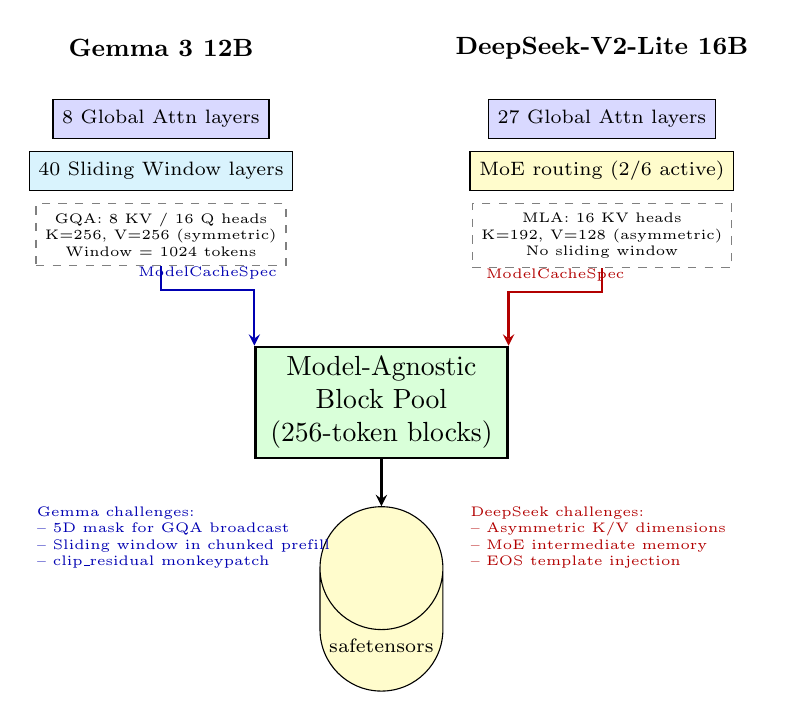
\begin{tikzpicture}[
    node distance=0.4cm,
    layer/.style={rectangle, draw=black, minimum width=2.4cm, minimum height=0.5cm, align=center, font=\scriptsize},
    pool/.style={rectangle, draw=black, thick, fill=green!15, minimum width=3.2cm, minimum height=1.2cm, align=center},
    spec/.style={rectangle, draw=gray, dashed, minimum width=2.6cm, minimum height=0.7cm, align=center, font=\tiny},
    arrow/.style={->, >=stealth, thick},
    label/.style={font=\scriptsize}
]

% Gemma 3 stack (left)
\node[font=\small\bfseries] (gemma_title) at (-2.8, 4.5) {Gemma 3 12B};

\node[layer, fill=blue!15] (g_global) at (-2.8, 3.6) {8 Global Attn layers};
\node[layer, fill=cyan!15, below=0.15cm of g_global] (g_slide) {40 Sliding Window layers};
\node[spec, below=0.15cm of g_slide] (g_spec) {GQA: 8 KV / 16 Q heads\\K=256, V=256 (symmetric)\\Window = 1024 tokens};

% DeepSeek stack (right)
\node[font=\small\bfseries] (ds_title) at (2.8, 4.5) {DeepSeek-V2-Lite 16B};

\node[layer, fill=blue!15] (d_global) at (2.8, 3.6) {27 Global Attn layers};
\node[layer, fill=yellow!20, below=0.15cm of d_global] (d_moe) {MoE routing (2/6 active)};
\node[spec, below=0.15cm of d_moe] (d_spec) {MLA: 16 KV heads\\K=192, V=128 (asymmetric)\\No sliding window};

% Shared Block Pool (center bottom)
\node[pool] (bp) at (0, 0) {Model-Agnostic\\Block Pool\\(256-token blocks)};

% ModelCacheSpec arrows
\draw[arrow, blue!70!black] (g_spec.south) -- ++(0,-0.3) -| node[pos=0.25, above, font=\tiny] {ModelCacheSpec} (bp.north west);
\draw[arrow, red!70!black] (d_spec.south) -- ++(0,-0.3) -| node[pos=0.25, above, font=\tiny] {ModelCacheSpec} (bp.north east);

% Disk below
\node[cylinder, draw=black, fill=yellow!20, minimum width=1.5cm, minimum height=0.8cm, shape border rotate=90, font=\scriptsize, below=0.6cm of bp] (disk) {safetensors};
\draw[arrow] (bp) -- (disk);

% Key differences annotations
\node[font=\tiny, align=left, text=blue!70!black, anchor=north west] at (-4.5, -1.2) {
    Gemma challenges:\\
    -- 5D mask for GQA broadcast\\
    -- Sliding window in chunked prefill\\
    -- clip\_residual monkeypatch
};

\node[font=\tiny, align=left, text=red!70!black, anchor=north east] at (4.5, -1.2) {
    DeepSeek challenges:\\
    -- Asymmetric K/V dimensions\\
    -- MoE intermediate memory\\
    -- EOS template injection
};

\end{tikzpicture}
\caption{Architecture comparison. The block pool abstracts away architectural differences through ModelCacheSpec. Gemma 3 uses grouped-query attention with hybrid sliding-window layers, requiring 5D mask expansion and window-aware chunked prefill. DeepSeek uses multi-latent attention with asymmetric K/V dimensions (192 vs 128) and MoE routing, requiring larger memory budgets for intermediate tensors.}
\label{fig:archcomp}
\end{figure}


Figure~\ref{fig:archcomp} compares the two model architectures. Gemma~3 uses hybrid attention (8 global + 40 sliding window layers) with symmetric KV dimensions. DeepSeek uses MLA with asymmetric dimensions (K=192, V=128). Both share the same block pool and Q4 pipeline via the ModelCacheSpec abstraction.

\subsection{Phase Timeline}

% Figure: Multi-Phase Cache Timeline — Prisoner's Dilemma
% Shows agent cache growth across 5 phases with TTFT annotations

\begin{figure}[t]
\centering
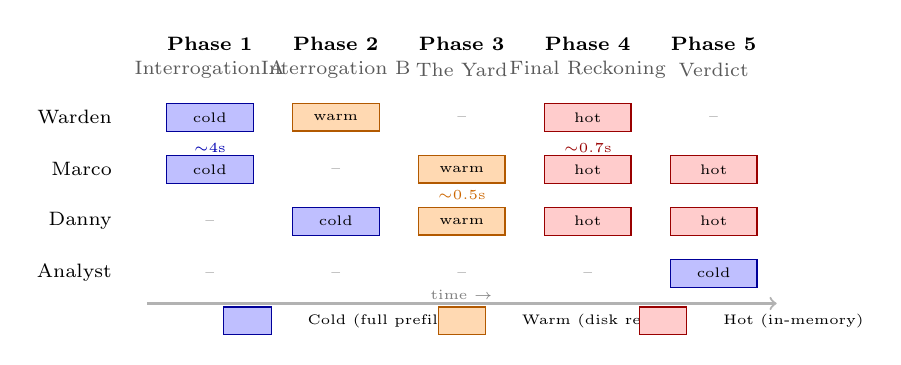
\begin{tikzpicture}[
    x=1.6cm, y=0.55cm,
    phase/.style={rectangle, draw=black, fill=gray!8, minimum height=2.4cm, align=center, font=\scriptsize},
    agent/.style={rectangle, minimum height=0.35cm, font=\tiny, align=center},
    cold/.style={fill=blue!25, draw=blue!60!black},
    warm/.style={fill=orange!30, draw=orange!70!black},
    hot/.style={fill=red!20, draw=red!60!black},
    ttft/.style={font=\tiny, text=black},
    label/.style={font=\scriptsize\bfseries}
]

% Phase labels
\foreach \i/\name/\short in {
    0/{Phase 1}/{\scriptsize Interrogation A},
    1/{Phase 2}/{\scriptsize Interrogation B},
    2/{Phase 3}/{\scriptsize The Yard},
    3/{Phase 4}/{\scriptsize Final Reckoning},
    4/{Phase 5}/{\scriptsize Verdict}} {
    \node[label] at (\i, 5.2) {\name};
    \node[font=\tiny, text=gray!70!black] at (\i, 4.6) {\short};
}

% Agent rows (bottom to top): Warden, Marco, Danny, Analyst
\node[font=\scriptsize, anchor=east] at (-0.7, 3.5) {Warden};
\node[font=\scriptsize, anchor=east] at (-0.7, 2.3) {Marco};
\node[font=\scriptsize, anchor=east] at (-0.7, 1.1) {Danny};
\node[font=\scriptsize, anchor=east] at (-0.7, -0.1) {Analyst};

% Warden: phases 1, 2, 4
\node[agent, cold, minimum width=1.1cm] at (0, 3.5) {cold};
\node[agent, warm, minimum width=1.1cm] at (1, 3.5) {warm};
\node[agent, hot, minimum width=1.1cm] at (3, 3.5) {hot};
% Warden inactive in phase 3, 5
\node[font=\tiny, text=gray] at (2, 3.5) {--};
\node[font=\tiny, text=gray] at (4, 3.5) {--};

% Marco: phases 1, 3, 4, 5
\node[agent, cold, minimum width=1.1cm] at (0, 2.3) {cold};
\node[font=\tiny, text=gray] at (1, 2.3) {--};
\node[agent, warm, minimum width=1.1cm] at (2, 2.3) {warm};
\node[agent, hot, minimum width=1.1cm] at (3, 2.3) {hot};
\node[agent, hot, minimum width=1.1cm] at (4, 2.3) {hot};

% Danny: phases 2, 3, 4, 5
\node[font=\tiny, text=gray] at (0, 1.1) {--};
\node[agent, cold, minimum width=1.1cm] at (1, 1.1) {cold};
\node[agent, warm, minimum width=1.1cm] at (2, 1.1) {warm};
\node[agent, hot, minimum width=1.1cm] at (3, 1.1) {hot};
\node[agent, hot, minimum width=1.1cm] at (4, 1.1) {hot};

% Analyst: phase 5 only
\node[font=\tiny, text=gray] at (0, -0.1) {--};
\node[font=\tiny, text=gray] at (1, -0.1) {--};
\node[font=\tiny, text=gray] at (2, -0.1) {--};
\node[font=\tiny, text=gray] at (3, -0.1) {--};
\node[agent, cold, minimum width=1.1cm] at (4, -0.1) {cold};

% TTFT annotations (below agent boxes)
\node[ttft, text=blue!70!black] at (0, 2.8) {${\sim}4$s};
\node[ttft, text=orange!80!black] at (2, 1.7) {${\sim}0.5$s};
\node[ttft, text=red!60!black] at (3, 2.8) {${\sim}0.7$s};

% Legend
\node[agent, cold, minimum width=0.6cm] at (0.3, -1.2) {};
\node[font=\tiny, anchor=west] at (0.7, -1.2) {Cold (full prefill)};
\node[agent, warm, minimum width=0.6cm] at (2.0, -1.2) {};
\node[font=\tiny, anchor=west] at (2.4, -1.2) {Warm (disk reload)};
\node[agent, hot, minimum width=0.6cm] at (3.6, -1.2) {};
\node[font=\tiny, anchor=west] at (4.0, -1.2) {Hot (in-memory)};

% Time arrow
\draw[->, thick, gray!60] (-0.5, -0.8) -- (4.5, -0.8);
\node[font=\tiny, text=gray] at (2, -0.6) {time $\rightarrow$};

\end{tikzpicture}
\caption{Agent cache state across prisoner's dilemma phases. Permanent agents (Warden, Marco, Danny) start cold and transition to warm/hot as context accumulates via cross-phase injection. Each phase extends the cached prefix rather than re-computing. The Analyst appears only in Phase~5 (cold start). TTFT annotations show projected latency from Table~\ref{tab:ttft} at equivalent context lengths.}
\label{fig:timeline}
\end{figure}


Figure~\ref{fig:timeline} shows cache state transitions across the 5-phase prisoner's dilemma scenario. Permanent agents (Warden, Marco, Danny) accumulate warm/hot cache across phases. The ephemeral agent (Analyst) cold-starts in Phase~5 only.

\subsection{Wikipedia Routing Diagram}

% Figure: Wikipedia Multi-Agent Routing Architecture
% Shows user query → router → cached expert agents → synthesis

\begin{figure}[t]
\centering
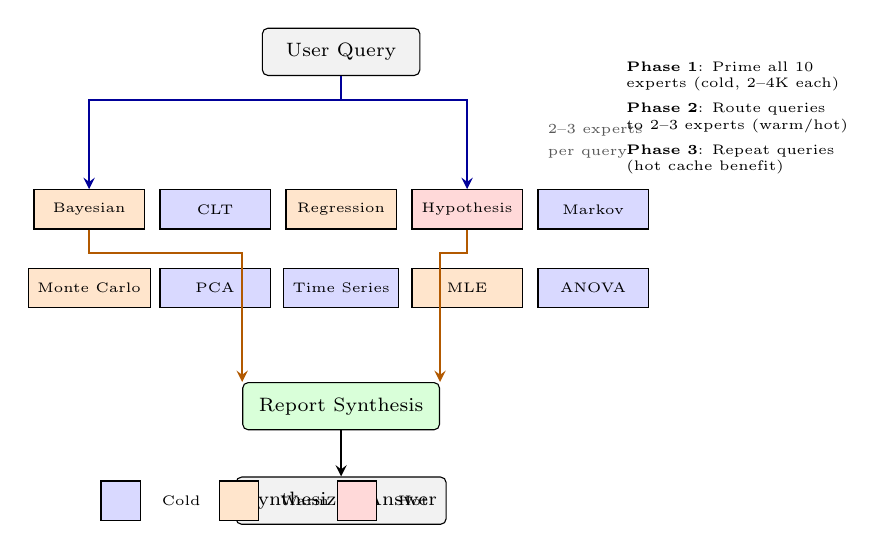
\begin{tikzpicture}[
    node distance=0.5cm,
    box/.style={rectangle, draw=black, rounded corners=2pt, minimum height=0.6cm, align=center, font=\scriptsize},
    expert/.style={rectangle, draw=black, minimum width=1.4cm, minimum height=0.5cm, align=center, font=\tiny},
    cold/.style={fill=blue!15},
    warm/.style={fill=orange!20},
    hot/.style={fill=red!15},
    arrow/.style={->, >=stealth, thick},
    label/.style={font=\tiny, text=gray!70!black}
]

% User query
\node[box, fill=gray!10, minimum width=2cm] (user) at (0, 3.5) {User Query};

% Expert agents grid (2 rows of 5)
\foreach \i/\name/\state in {
    0/Bayesian/warm,
    1/CLT/cold,
    2/Regression/warm,
    3/Hypothesis/hot,
    4/Markov/cold} {
    \node[expert, \state] (e\i) at (\i*1.6 - 3.2, 1.5) {\name};
}
\foreach \i/\name/\state in {
    5/Monte Carlo/warm,
    6/PCA/cold,
    7/Time Series/cold,
    8/MLE/warm,
    9/ANOVA/cold} {
    \pgfmathsetmacro{\x}{(\i-5)*1.6 - 3.2}
    \node[expert, \state] (e\i) at (\x, 0.5) {\name};
}

% Article cache indicators (small boxes below experts)
\foreach \i in {0,...,9} {
    \pgfmathsetmacro{\y}{ifthenelse(\i<5, 1.1, 0.1)}
    \pgfmathsetmacro{\x}{ifthenelse(\i<5, \i*1.6-3.2, (\i-5)*1.6-3.2)}
}

% Arrows from user to relevant experts (highlighted)
\draw[arrow, blue!60!black] (user.south) -- ++(0,-0.3) -| (e0.north);
\draw[arrow, blue!60!black] (user.south) -- ++(0,-0.3) -| (e3.north);

% Label: "2--3 experts per query"
\node[label, anchor=west] at (2.5, 2.5) {2--3 experts};
\node[label, anchor=west] at (2.5, 2.2) {per query};

% Synthesis agent
\node[box, fill=green!15, minimum width=2.5cm] (synth) at (0, -1.0) {Report Synthesis};

% Arrows from selected experts to synthesis
\draw[arrow, orange!70!black] (e0.south) -- ++(0,-0.3) -| (synth.north west);
\draw[arrow, orange!70!black] (e3.south) -- ++(0,-0.3) -| (synth.north east);

% Output
\node[box, fill=gray!10, minimum width=2cm] (out) at (0, -2.2) {Synthesized Answer};
\draw[arrow] (synth) -- (out);

% Phase annotations on right
\node[font=\tiny, align=left, anchor=north west] at (3.5, 3.5) {
    \textbf{Phase 1}: Prime all 10\\
    experts (cold, 2--4K each)\\[3pt]
    \textbf{Phase 2}: Route queries\\
    to 2--3 experts (warm/hot)\\[3pt]
    \textbf{Phase 3}: Repeat queries\\
    (hot cache benefit)
};

% Legend
\node[expert, cold, minimum width=0.5cm] at (-2.8, -2.2) {};
\node[font=\tiny, anchor=west] at (-2.4, -2.2) {Cold};
\node[expert, warm, minimum width=0.5cm] at (-1.3, -2.2) {};
\node[font=\tiny, anchor=west] at (-0.9, -2.2) {Warm};
\node[expert, hot, minimum width=0.5cm] at (0.2, -2.2) {};
\node[font=\tiny, anchor=west] at (0.6, -2.2) {Hot};

\end{tikzpicture}
\caption{Wikipedia multi-agent routing. Ten expert agents are primed with article content (cold prefill). Cross-topic queries route to 2--3 relevant experts whose caches are warm/hot from priming. A reporter agent synthesizes responses. Repeated queries to the same experts benefit from hot cache (projected 10--30$\times$ TTFT reduction vs cold).}
\label{fig:wikirouting}
\end{figure}


Figure~\ref{fig:wikirouting} shows the 3-phase routing protocol. Phase~1 primes 10 experts with cold-start prefill. Phase~2 routes cross-topic queries to 2--3 warm experts each. Phase~3 re-queries hot experts.

\end{document}
